\clearpage
\phantomsection

\setcounter{chapter}{0}
\chapter[{GIỚI THIỆU BÀI TOÁN}]{Giới thiệu bài toán}

Đoạn giới thiệu chương: trình bày mục đích, nội dung của chương này. 

\vspace{0.3cm}

\section{Mục lớn trong chương}

abcabc

\subsection{Mục nhỏ trong chương}


List item sẽ như thế này:

\renewcommand{\labelitemi}{$-$}
\begin{itemize}
	\item \textit{gạch đầu dòng 1}: Nội dung của gạch đầu dòng 1.
	\item \textit{gạch đầu dòng 2}: ...
	\item \textit{gạch đầu dòng 3}: ...
\end{itemize} 
\vspace{0.3cm}

% Thêm một chút Khoảng trống nếu cần
\vspace{0.3cm}




Chèn hình ảnh, các hình ảnh để trong thư mục /figures: 

Hình ảnh bình thường:
\begin{figure} [!htb]
	\centering
    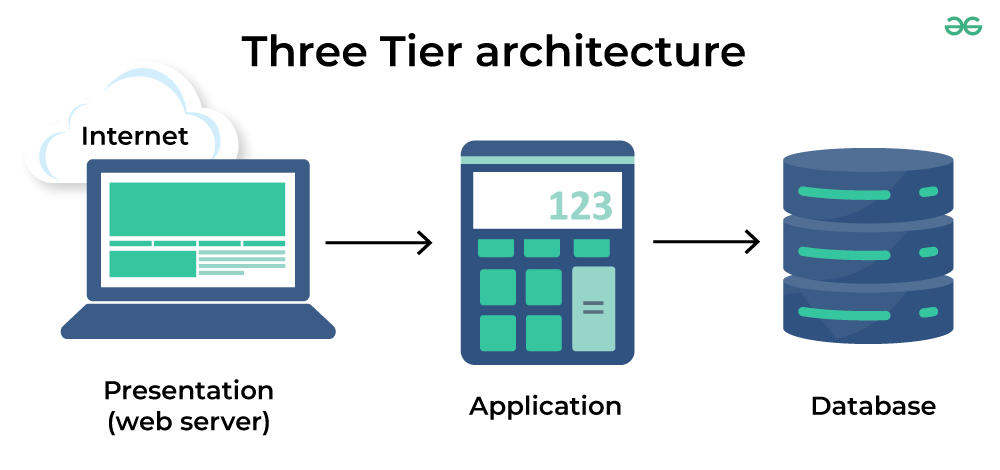
\includegraphics[width=1\linewidth]{figures/three-tier-architecture.png}
	\caption{Caption của ảnh 1}
	\label{fig:UET_logo2}
\end{figure}

% Thêm float barrier để ngăn chặn các hình ảnh tràn ra ngoài chương
\FloatBarrier


Hình ảnh được xoay dọc (với những hình ảnh có chiều ngang quá lớn, nếu để ngang chữ sẽ bị bé, bị vỡ ảnh hoặc không nhìn rõ):

\begin{figure} [!htb]
	\centering
	\rotatebox{90}{
        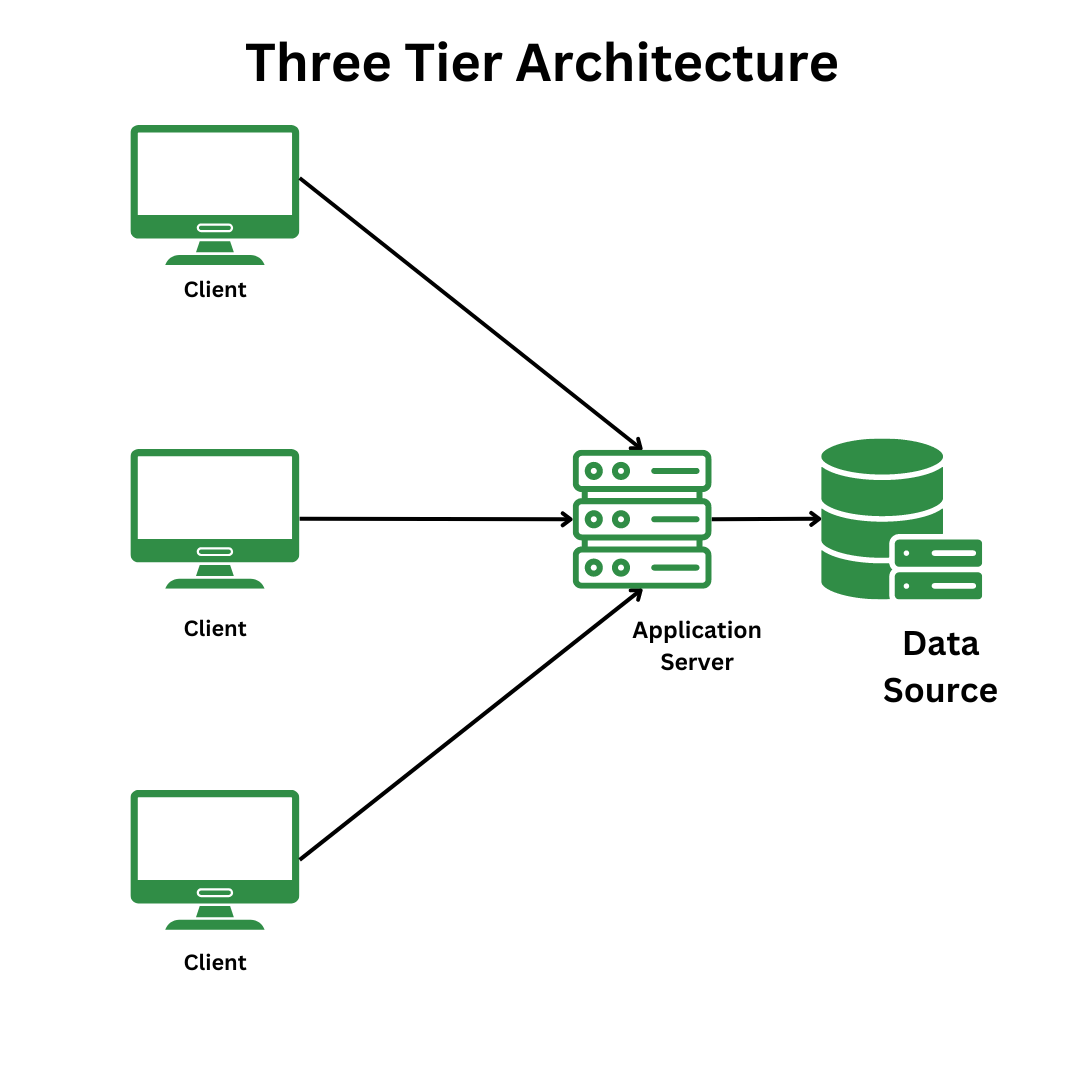
\includegraphics[width=0.5\linewidth]{figures/three-tier-architecture-2.png}
    }
	\caption{Caption của ảnh 2}
	\label{fig:UET_logo}
\end{figure}

% Thêm float barrier để ngăn chặn các hình ảnh tràn ra ngoài chương
\FloatBarrier

\vspace{1cm}

\textbf{Trích dẫn:} Các mục trích dẫn viết trong file main.tex, các trích dẫn viết theo chuẩn IEEE, khi muốn trích dẫn thì viết như này \cite{Cockburn2005}



\begin{landscape}
	\noindent Bảng biểu

	\begin{longtable}{|>{\raggedright\arraybackslash}m{4cm}|>{\raggedright\arraybackslash}m{4.5cm}|>{\raggedright\arraybackslash}m{4.5cm}|>{\raggedright\arraybackslash}m{4.5cm}|>{\raggedright\arraybackslash}m{4.5cm}|}
	\caption{Caption của bảng} \\
	\hline
	\textbf{Tính năng} & \textbf{Hệ thống} & \textbf{Đối thủ 1} & \textbf{Đối thủ 2} & \textbf{Đối thủ 3} \\
	\hline
	Tính năng 1 & x & x & x & x \\
	\hline
	Tính năng 2 & x & x & x & x \\
	\hline
	Tính năng 3 & x & x & x & x \\
	\hline
	Tính năng 4 & x & x & x & x \\
	\hline

\end{longtable}
\end{landscape}



\vspace{0.3cm}


Đoạn kết luận chương: tóm tắt lại nội dung của chương này, dẫn dắt vào nội dung chương tiếp theo.